ROM, Read Only Memory, kan brukes i enkodere når man ønsker en bestem relasjon
mellom input og output.
Man lager et map som relaterer spesifikke input til spesifikke output.

\paragraph{7-Segment} \mbox{} \\
Et 7-segment, som brukes til å vise et siffer, styres av 7 input pinner.
Den har 7 streker som kan lyse for å vise forksjellige siffer.

\begin{figure}[H]
  \caption{7-Segment med pins}
  \centering
  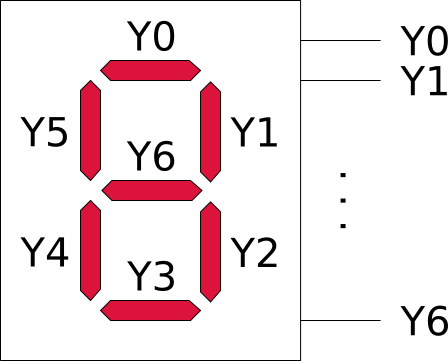
\includegraphics[width=0.5\textwidth]{./img/7-segment}
\end{figure}

Forholdet mellom et input og hvilke streker som skal lyse bestemmes av en ROM.

\begin{figure}[H]
  \caption{7-Segment med pins}
  \centering
  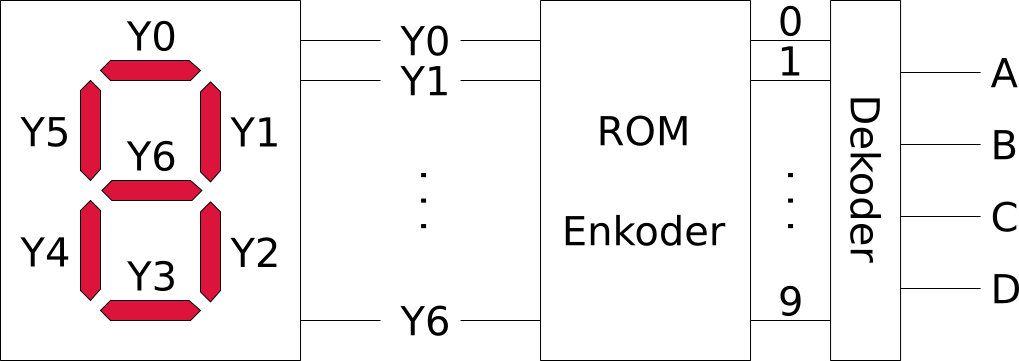
\includegraphics[width=\textwidth]{./img/7-segment-rom}
\end{figure}

Når input er lik 0 vil vi at alle streker bortsett fra den i midten skal lyse.
Når input er lik 1 vil vi at kun de to høyre strekene skal lyse, osv...

Vi kan programmere ROMen til å gi oss den mappingen vi ønsker.

\begin{table}[H]
  \centering
  \begin{tabular}{c c c c c c c c c c c}
    A & B & C & D & Y0 & Y1 & Y2 & Y3 & Y4 & Y5 & Y6 \\ \hline
    0 & 0 & 0 & 0 &  1 &  1 &  1 &  1 &  1 &  1 &  0 \\
    0 & 0 & 0 & 1 &  0 &  1 &  1 &  0 &  0 &  0 &  0 \\
    . &   &   &   &    &    &    &    &    &    &    \\
    . &   &   &   &    &    &    &    &    &    &    \\
    . &   &   &   &    &    &    &    &    &    &    \\
    1 & 0 & 0 & 0 &  1 &  1 &  1 &  1 &  1 &  1 &  1 \\
    1 & 0 & 0 & 1 &  1 &  1 &  1 &  0 &  0 &  1 &  1
  \end{tabular}
\end{table}
